
\section{Anderson lattice-model and Heavy Fermion systems}

Assume a metal where we have introduced so many magnetic impurities that we cannon treat them as isolated impurities anymore. We are therefore looking at a itinerant electron-system, coupled to a lattice of Kondo-type impurities, similar to the impurities in the last section. The system is then described by the Anderson lattice-model: 

\begin{align*}
    H = \sum_{k\sigma} \ep_k \cd_{k\sigma}c_{k\sigma} + E_0 \sum_{i\sigma} \Fd_{i\sigma} F_{i\sigma} + U\sum_i \Fd_{i \uparrow} F_{i \uparrow} \Fd_{i \downarrow} F_{i \downarrow} \\ 
    + \sum_{ik\sigma} V_{k\sigma i} \left(\cd_{k\sigma}F_{i\sigma} + \Fd_{i\sigma}c_{k\sigma}\right)
\end{align*}

this is also a complicated problem, due to the $U$-term. We set $U = \infty$, as we did before, which means no-double occupancy constraint on each lattice site $i$. The number of lattice sites are constant, whereas the number of occupants can vary. We define new fermionic and bosonic operators, similarly to what we did before 

\begin{align*}
    \Fd_{i\sigma} = \fd_{i\sigma}b_i \\ 
    F_{i\sigma} = f_{i\sigma} \bd_i. 
\end{align*}

We therefore have an extra boson-field, $b_i$, similar to what we had in the impurity problem, but now for each lattice site $i$. From this, we get 

\begin{align*}
    \sum_\sigma \Fd_{i\sigma} F_{i\sigma} \leq 1 \\
    \implies Q_i \equiv \sum_\sigma \fd_{i\sigma}f_{i\sigma} + \bd_i  b_i = 1. 
\end{align*}

The partition function for $U = \infty$: 

\begin{align*}
    Z = \int \D \cd \D c \D \fd \D f \D \bd \D b \left(\prod_{i\tau} \delta_{Q_i, 1} \right) \e^S \\ 
    S = -\sum_{i\sigma} \int_{0}^{\beta} \dd \tau \left[ \bd_i \pdv{b_i}{\tau} + \fd_{i\sigma}(\partial_\tau + E_0)f_{i\sigma} \right] - \sum_{k\sigma} \int_{0}^{\beta} \dd \tau \cd_{k\sigma}(\partial_\tau + \ep_k)c_{k\sigma} \\ 
    - \sum_{k\sigma i} \int_{0}^{\beta} \dd \tau V_{k\sigma i}\left( \cd_{k\sigma} \bd_i f_{i\sigma} + \fd_{i\sigma}c_{k\sigma} b_i \right) 
\end{align*}

where we have imposed the constraint on both imaginary time $\tau$ and the lattice points $i$. 

\begin{align*}
    \prod_{i\tau} \delta_{Q_i, 1} = \prod_{i\tau} \int_{-\pi}^{\pi} \frac{\dd \lambda_i}{2\pi}\e^{-i\sum_i  \int_{0}^{\beta} \dd \tau \lambda_i(Q_i - 1) }.
\end{align*}


Thus we get, as in the impurity problem, an un-constrained partition function, 
\begin{align*}
    Z = \int \D \cd \D c \D \fd \D f \D \bd \D b \D \lambda \e^{\Tilde{S}} \\ 
    \Tilde{S} = -\sum_{i\sigma} \int_{0}^{\beta} \dd \tau \left[ \bd_i \pdv{b_i}{\tau} + \fd_{i\sigma}(\partial_\tau + E_0)f_{i\sigma} \right] - \sum_{k\sigma} \int_{0}^{\beta} \dd \tau \cd_{k\sigma}(\partial_\tau + \ep_k)c_{k\sigma} \\ 
    - \sum_{k\sigma i} \int_{0}^{\beta} \dd \tau V_{k\sigma i}\left( \cd_{k\sigma} \bd_i f_{i\sigma} + \fd_{i\sigma}c_{k\sigma} b_i \right) - \sum_i \int_{0}^{\beta} \dd \tau i\lambda_i \left(\sum_\sigma \fd_{i\sigma}f_{i\sigma} + \bd_i  b_i - 1\right) \\
    = \sum_i \int_{0}^{\beta} \dd \tau i\lambda_i -\sum_{i\sigma} \int_{0}^{\beta} \dd \tau \left[ \bd_i (\partial_\tau + i\lambda_i)b_i  + \fd_{i\sigma}(\partial_\tau + E_0 + i\lambda_i)f_{i\sigma} \right]  \\- \sum_{k\sigma} \int_{0}^{\beta} \dd \tau \cd_{k\sigma}(\partial_\tau + \ep_k)c_{k\sigma}  
    - \sum_{k\sigma i} \int_{0}^{\beta} \dd \tau V_{k\sigma i}\left( \cd_{k\sigma} \bd_i f_{i\sigma} + \fd_{i\sigma}c_{k\sigma} b_i \right).
\end{align*}

Mean field: 

\begin{align*}
    i\lambda_i \to \lambda \quad \quad b_i \to b \quad \quad E_o + i\lambda \to E_0 + \lambda \equiv \ep_f 
\end{align*}

The the action becomes 

\begin{align*}
    \Tilde{S} = N\beta\lambda - N\beta \lambda b^2 - \sum_{i\sigma} \int_{0}^{\beta} \dd \tau \fd_{i\sigma}(\partial_\tau + \ep_f)f_{i\sigma} - \sum_{k\sigma} \int_{0}^{\beta} \dd \tau \cd_{k\sigma}(\partial_\tau + \ep_k)c_{k\sigma} \\ 
    - \sum_{k\sigma i} \int_{0}^{\beta} \dd \tau  V_{k\sigma i}b\left( \cd_{k\sigma}f_{i\sigma} + \fd_{i\sigma}c_{k\sigma}\right), 
\end{align*}

where $N$ is the volume, i.e. the number of impurity lattice sites, of the system. Now we approximate the coupling term and Fourier transform the k-part of the $f$-sector 

\begin{align*}
    \sum_{i\sigma} \int_{0}^{\beta} \dd \tau \fd_{i\sigma}(\partial_\tau + \ep_f)f_{i\sigma} \to \sum_{k\sigma} \int_{0}^{\beta} \dd \tau \fd_{k\sigma}(\partial_\tau + \ep_f)f_{k\sigma} \\
    - \sum_{k\sigma i} \int_{0}^{\beta} \dd \tau V_{k\sigma i}b\left( \cd_{k\sigma}f_{i\sigma} + \fd_{i\sigma}c_{k\sigma}\right) \to - \sum_{k\sigma} \int_{0}^{\beta} \dd \tau Vb\left( \cd_{k\sigma}f_{k\sigma} + \fd_{k\sigma}c_{k\sigma}\right). 
\end{align*}

When we write the model like this, it is essentially a Fourier transformed real-space model with unit cells consisting of $c-$ and $f-$electron orbitals. The $c-$electrons can jump, whereas the $f-$ electrons cannot, since they are dispersion-less. They become mobile, since they are coupled to the $c-$electrons via the matrix element $V$. 
\begin{align*}
    \sum_{ij\sigma} t_{cc}^{ij} \cd_{i\sigma} c_{j\sigma} \to \sum_{k\sigma} \ep_k \cd_{k\sigma} c_{k\sigma} \\ 
    E_0 \sum_i \Fd_{i\sigma} F_{i\sigma} \to E_0 \sum_k \Fd_{k\sigma} F_{k\sigma} \\
    V \sum_i \left( \cd_i F_i + \Fd_i c_i \right) \to V\sum_{k\sigma} \left( \cd_{k\sigma} F_{k\sigma} + \Fd_{k\sigma} c_{k\sigma} \right)
\end{align*}

and there are as many lattice sites for the electrons as there are for the impurities. Then we get, in mean field theory \\

\begin{align*}
    Z = \e^{-N\beta \lambda (b^2 - 1)} \int \D \psi^\dagger \D \psi \e^{S_{MF}} \\ 
    S_{MF} = -\sum_{k\sigma} \int_{0}^{\beta} \dd \tau \psi^\dagger_{k\sigma}A\psi_{k\sigma} \\ 
    \psi_{k\sigma} = \begin{pmatrix} c_{k\sigma} \\ f_{k\sigma} \end{pmatrix} \\
    A = \begin{pmatrix} \partial_\tau + \ep_k && Vb \\
    Vb && \partial_\tau + \ep_f \end{pmatrix} 
\end{align*}

\begin{align*}
    Z = \e^{-N\beta \lambda (b^2 - 1)} \e^{\Tr\ln A} 
\end{align*} 
\begin{align*}
    \Tr \ln A = \sum_{k\sigma} \int_{0}^{\beta} \dd \tau \tr \ln \begin{pmatrix} \partial_\tau + \ep_k && Vb \\
    Vb && \partial_\tau + \ep_f \end{pmatrix} \\ 
    = \frac{1}{\beta}\sum_{\omega_n}\sum_{k \sigma} \int_{0}^{\beta} \dd \tau \tr \ln \begin{pmatrix} -i\omega_n + \ep_k && Vb \\
    Vb && -i\omega_n + \ep_f \end{pmatrix} \\
    = \sum_{\omega_n}\sum_{k \sigma} \ln(i\omega_n - E_k^+)(i\omega_n - E_k^-) = 2\sum_k \ln\left[\left(1 + \e^{-\beta E_k^+}\right)\left(1 + \e^{-\beta E_k^-}\right)\right] \\
    E_k^{\pm} = \frac{1}{2}\left( \ep_k + \ep_f \pm \sqrt{(\ep_k - \ep_f)^2 +4V^2b^2} \right) \\
    f = N\lambda (b^2 - 1) - \frac{2}{\beta} \sum_k \left[ \ln \left(1 + \e^{-\beta E_k^+}\right)\ \ln\left(1 + \e^{-\beta E_k^-}\right) \right] 
\end{align*}

\begin{figure}
    \centering
    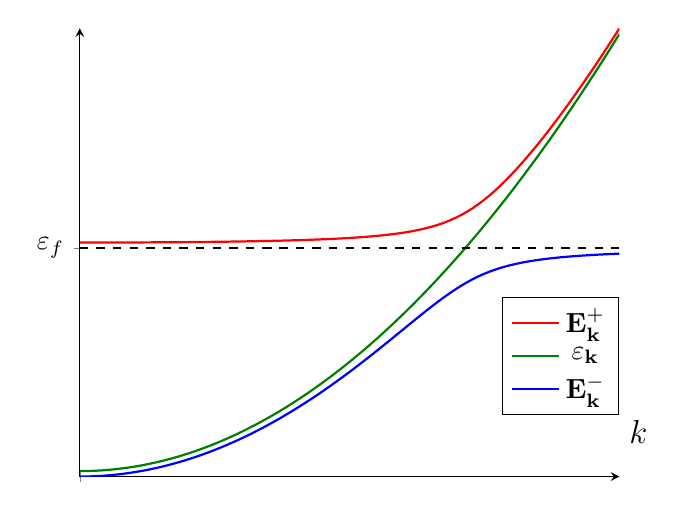
\begin{tikzpicture}
\begin{axis}[
    legend style={at={(1,0.4)}},
    ytick = {1},
    yticklabels = {$\varepsilon_f$},
    xtick = {0},
    xticklabels ={,,},
    xlabel = \large $k$,
    axis lines = left,
    x label style={at={(axis description cs:1,0.1)}, anchor = west},
    %y label style={at={(axis description cs:0.15,1)},rotate=-90,anchor=south},
    %xlabel = $x$,
    %sylabel = {$f(x)$},
]
%Below the red parabola is defined
\addplot [
    thick,
    domain=0:1.4, 
    samples=100, 
    color=red,
]{1/2 * (1 + x^2 + sqrt((x^2 - 1)^2 + 0.1))};


\addplot [
    thick,
    domain=0:1.4, 
    samples=100, 
    color=green!50!black,
]{x^2};

%Here the blue parabloa is defined
\addplot [
    thick,
    domain=0:1.4, 
    samples=100, 
    color=blue,
    ]{1/2 * (1 + x^2 - sqrt((x^2 - 1)^2 + 0.1))};


\addplot[
    thick,
    domain = 0:1.4,
    samples = 100,
    dashed
    ]{1};

\addlegendentry{$\mathbf{E_k^+}$}
\addlegendentry{$\mathbf{\varepsilon_k}$}
\addlegendentry{$\mathbf{E_k^-}$}
\end{axis}
\end{tikzpicture}
    \caption{How the dispersion relation changes when $V \ne 0$. NB: All the energy levels relative the Fermi-level.}
    \label{fig:my_label}
\end{figure}


Again this has the form of an electron gas plus a purely bosonic contribution. \\ 

We see that the dispersion relations close to the renormalized impurity-surface $(\ep_f)$ are very flat. This implies that the quasi-particles have a large effective mass. \\

\begin{align*}
    Z = Z_b \cdot Z_f \\
    Z_f = \int \D \psi^\dagger \D \psi e^S \\
    S = -\sum_{k\sigma} \int_{0}^{\beta} \dd \tau \psi^\dagger_{k\sigma} A \psi_{k\sigma} 
\end{align*}

This partition function is an effective free-fermion theory with the Hamilton-operator 

\begin{align*}
    H = \sum_{k\sigma} \psi_{k\sigma}^\dagger \begin{pmatrix} \ep_k && Vb \\
    Vb && \ep_f \end{pmatrix} \psi_{k\sigma} \\
    S = - \int_{0}^{\beta} \dd \tau \left[ \sum_{k\sigma} \psi_{k\sigma}^\dagger \pdv{\psi_{k\sigma}^\dagger}{\tau} + \psi_{k\sigma}^\dagger H \psi_{k\sigma} \right] \\ = \sum_{k\sigma} \varphi_{k\sigma}^\dagger \pdv{\varphi_{k\sigma}^\dagger}{\tau} + \varphi_{k\sigma}^\dagger D \varphi_{k\sigma} \\
    H = \sum_{k\sigma} E_k^+\varphi_{k\sigma, +}^{\dagger} \varphi_{k\sigma, +} + E_k^- \varphi_{k\sigma, -}^\dagger \varphi_{k\sigma, -} 
\end{align*}

\begin{align*}
    \varphi_{k\sigma} = \begin{pmatrix} \varphi_{k\sigma, +}  \\ \varphi_{k\sigma, -} \end{pmatrix} \quad D = \begin{pmatrix} E_k^+ && 0 \\ 0 && E_k^- \end{pmatrix} 
    %Karl p. 222
\end{align*}

Where we have diagonalized the Hamiltonian. Even when $U \to \infty$, the system is a renormalized free electron gas, maybe with heavy electrons! \\ 

In the last section, we proved that $\ep_f$ was nailed to the Fermi-surface

\begin{align*}
    \ep_f = D \e^{-\frac{\pi \abs{E_0}}{2\Delta_0}} \quad \Delta_0 = \pi \rho_0 V^2. 
\end{align*}

Is this the case in this lattice model? To answer this question, we must solve the stationary point equation. \\

The physics of the system is determined at the Fermi-surface, or very near. If $\ep_f$ is nailed to the Fermi-surface in this case as well, the low-energy excitations (i.e. most important fluctuations) will have a large effective mass: $E_k^\pm$ is flat near $\ep_f$. We get a heavy-fermion system from correlation effects, because $\ep_f \approx \ep_F$ when $U$ is large. \\

Before moving on to the stationary point condition, we will have a look at the propagators of the system. \\ 

Fermion propagator: 

\begin{align*}
    \psi_{k\sigma} = \begin{pmatrix} c_{k\sigma} \\ f_{k\sigma} \end{pmatrix} \\ 
    G(\tau, \ep_k, \ep_f) = -\expval{\psi_{k\sigma} \psi_{k\sigma}^\dagger} \\ 
    G^{-1}(\tau, \ep_k, \ep_f) = -A = - \begin{pmatrix} \partial_\tau +\ep_k && Vb \\ Vb && \partial_\tau + \ep_f \end{pmatrix} \\ 
    G^{-1}(k, i\omega_n) = - \begin{pmatrix} -i\omega_n +\ep_k && Vb \\ Vb && -i\omega_n + \ep_f \end{pmatrix} \\
    G(k, i\omega_n) = \frac{1}{\det G^{-1}} \begin{pmatrix} i\omega_n - \ep_k && Vb \\ Vb && i\omega_n - \ep_f \end{pmatrix}
\end{align*}

\begin{align*}
    \det G^{-1} = (i\omega_n - \ep_k)(i\omega_n - \ep_f) - s_0^2 = (i\omega_n - E_k^+)(i\omega_n - E_k^-) \\ 
    E_k^\pm = \frac{1}{2}\left(\ep_k + \ep_f \pm \sqrt{(\ep_k - \ep_f)^2 + 4s_0^2}\right)
\end{align*}

\begin{align*}
    G_{cc}(k,i\omega_n) = -\expval{c_{k\sigma} c_{k\sigma}^\dagger} = \frac{i\omega_n - \ep_f}{(i\omega_n - E_k^+)(i\omega_n - E_k^-)} \\ 
    G_{ff}(k,i\omega_n) = -\expval{f_{k\sigma} f_{k\sigma}^\dagger} = \frac{i\omega_n - \ep_k}{(i\omega_n - E_k^+)(i\omega_n - E_k^-)}
\end{align*}

\begin{align*}
    G_{cf} = G_{fc} = -\expval{c_{k\sigma} f_{k\sigma}^\dagger} = \frac{s_0}{(i\omega_n - E_k^+)(i\omega_n - E_k^-)} = 0 \quad (V = 0).
\end{align*}

When the hybridization term is $0$, the vertices connecting $c-$ and $f-$field are $0$, and hence the probability of a $c-$fermion changing to a $f-$fermion is 0. \\ 

$V = 0$: 

\begin{align*}
    G_{cc}(k,i\omega_n) = -\expval{c_{k\sigma} c_{k\sigma}^\dagger} = \frac{i\omega_n - \ep_f}{(i\omega_n - \ep_k)(i\omega_n - \ep_f)} = \frac{1}{i\omega_n - \ep_k} \\ 
    G_{ff}(k,i\omega_n) = -\expval{f_{k\sigma} f_{k\sigma}^\dagger} = \frac{i\omega_n - \ep_k}{(i\omega_n - \ep_k)(i\omega_n - \ep_f)} = \frac{1}{i\omega_n - \ep_f}
\end{align*}

In this case, the $f-$fermions are dispersionless, which means that they are localized, as expected. The effect of $U$ is only present in $G_{ff}$: $E_0 \to \ep_f$. We can write these propagators on Fermi-liquid form, even when $V \neq 0$. We show this looking at $G_{cc}$:

\begin{align*}
    G_{cc}(k,i\omega_n) = -\expval{c_{k\sigma} c_{k\sigma}^\dagger} = \frac{i\omega_n - \ep_f}{(i\omega_n - E_k^+)(i\omega_n - E_k^-)} = \frac{A}{i\omega_n - E_k^+} + \frac{B}{i\omega_n - E_k^-} \\
    \implies (A + B)i\omega_n - (BE_k^^+ + AE_k^-) = i\omega_n - \ep_f. 
\end{align*}

By using $A + B = 1$, we get the following expressions for $A$ and $B$ using the equation above. 

\begin{align*}
    A = \frac{1}{2}\left( 1 + \frac{\ep_k - \ep_f}{\sqrt{(\ep_k - \ep_f)^2 + 4s_0^2}}\right) \quad B = \frac{1}{2}\left( 1 - \frac{\ep_k - \ep_f}{\sqrt{(\ep_k - \ep_f)^2 + 4s_0^2}}\right)
\end{align*}

In the limit $s_0 \ll \abs{\ep_k - \ep_f}$, we get $A \approx 1, B \approx 0$. And in the limit $s_0 \ll \abs{\ep_k - \ep_f}, \ep_k - \ep_f < 0$, we get the opposite. In addition, $E_k^+ \approx \ep_k$ and $E_k^- \approx \ep_f$ under these considerations, and we get the desired Fermi-liquid (simple pole) form in both cases

\begin{align*}
    G_{cc}(k,i\omega_n) \approx \frac{1}{i\omega_n - \ep_k} \quad
    G_{ff}(k,i\omega_n) \approx \frac{1}{i\omega_n - \ep_f}, \quad \ep_k - \ep_f > 0 \\
    G_{cc}(k,i\omega_n) \approx \frac{1}{i\omega_n - \ep_f} \quad
    G_{ff}(k,i\omega_n) \approx \frac{1}{i\omega_n - \ep_k}, \quad \ep_k - \ep_f < 0. 
\end{align*}

Free energy per unit cell: 

\begin{align*}
    f = -\lambda(1-b^2) - \frac{2}{\beta N} \sum_k \ln\left(1 + \e^{-\beta E_k^+} \right) \ln\left(1 + \e^{-\beta E_k^-} \right) \\ 
    = -(\ep_f - E_0)\left( 1 - \frac{\Delta}{\Delta_0} \right) - \frac{2}{\beta N} \sum_k \ln\left(1 + \e^{-\beta E_k^+} \right) \ln\left(1 + \e^{-\beta E_k^-} \right), 
 \end{align*}
where N is the number of unit cells/lattice points. 
\begin{align*}
    \pdv{f}{\ep_f} = 0 = -1 + \frac{\Delta}{\Delta_0} + \frac{2}{N}\sum_k \left[ \pdv{E_k^-}{\ep_f}f(E_k^-) + \pdv{E_k^+}{\ep_f}f(E_k^+)\right] \\ 
    \pdv{f}{\Delta} = 0 = \frac{\ep_f - E_0}{\Delta_0} + \frac{2}{N} \sum_k \left[ \pdv{E_k^-}{\Delta}f(E_k^-) + \pdv{E_k^+}{\Delta}f(E_k^+)\right] \\ 
    -\pdv{f}{\mu} = \frac{2}{N}\sum_k \left[ f(E_k^-) + f(E_k^+) \right] = n = n_f + n_c. 
\end{align*}
The Kondo limit: 
\begin{align*}
    n_f = 1 - \frac{\Delta}{\Delta_0} \approx 1 \\ 
    \frac{\ep_f - E_0}{\Delta_0} + 2\sum_{k<k_F}\frac{-1}{\pi \rho_0} \frac{1}{\sqrt{(\ep_k - \ep_f)^2 + s_0^2}} = 0 \\
    \frac{\ep_f - E_0}{\Delta_0} \approx \frac{-2}{2D}\int_{-D}^{\mu} \frac{\dd \ep}{\ep - \ep_f} = -\frac{1}{D}\ln\left(\frac{\mu - \ep_f }{-D - \ep_f}\right) \\ 
    \approx -\frac{1}{D}\ln\left(\frac{\ep_f - \mu}{D}\right) = -2\rho_0 \ln\left(\frac{\ep_f - \mu}{D}\right)
\end{align*}

$\ep_f \ll E_0$: 

\begin{align*}
    -\frac{\pi \abs{E_0}}{2\Delta_0} \approx \ln \left( \frac{T_K}{D}\right) \\
    T_K = D\e^{-\frac{\pi \abs{E_0}}{2\Delta_0}}
\end{align*}

$\ep_f$ near the Fermi-level implies that the quasi-particles have a large effective mass, typically in the range $m^* \approx 1000m$ when $U \to \infty$. \\ 

From this analysis, we can conclude that the system is effectively an electron gas with strongly renormalized quasi-particles. The quasi-particles are a linear combination of $c-$ and $f-$ fermions. The larger the value of $\abs{E_0}$, the smaller the difference $\ep_f - \ep_F$ becomes. Since the $f-$fermions originally were localized, i.e. effectively infinite mass, the quasi-particles become more and more heavy as $\abs{E_0}$ increase. In the Kondo regime, the mass becomes extremely large, $m^* \approx 1000m$. Even tho the mass becomes so large, the Fermi-liquid picture survives in $d = 3$. If $U = 0$, this effect vanishes, because the renormalization of the f-level wouldn't have taken place. \\

In the past sections, we've looked at a few examples of what is known as bosonization of fermion-theories, some with weak attractive interactions and some with strong repulsive interactions. 

\begin{itemize}
    \item Weak attractive interactions: BCS-theory, unstable electron gass picture.
    \item Strong repulsive interactions between fermions: Hubbard model, Anderson model, Anderson models, Kondo model. In these cases, the systems renormalize to free electron gasses even in the limit $U \to \infty$. They are Fermi liquids. In the next sections, we will have a look bosonization of 1-dimensional systems. We will see that arbitratily small interactions in these cases will destroy the Fermi-picture. The systems becomes a new type of metallic system - a new renormalization fixpoint called Luttinger liquid! Here the fermionic, single-particle picture we are intuitively familiar with is completely altered into a picture dominated by effective bosons, rather than fermions. There are no single-particle excitations, only collective bosonic excitations. 
\end{itemize}
